\documentclass[a4paper]{article}

\usepackage[english]{babel}
\usepackage[utf8]{inputenc}
\usepackage{graphicx}
\usepackage{collection}

\title{Collection \TeX}

\author{E. Fedotov, M. Douglass, J. Chin}

\date{\today}

\begin{document}
\maketitle

\section{Motivation}
This package was made to serve two purposes. First, a collection of diagrams is included for demonstration. Second, this doc is meant to be a guide for someone new to publishing \LaTeX 
books. The majority necessary to get started should be provided here. 

\section{The Diagrams}
\subsection{Stacks}
Generally, most of these can be applied to any array-like diagrams.
\subsection{Environment}
\textbf{stack}: The environment \textbf{stack} can be used to draw any data structure that involves cells.\vspace{3mm}\\
\verb!\begin{stack}{<required>}!\\
\verb!  ...!\\
\verb!\end{stack}!

\subsection{Required Options}
\textbf{vertical}: The option \textbf{vertical} is used to draw a sequence of vertical cells.\vspace{3mm}
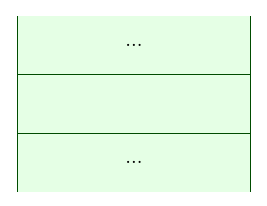
\includegraphics[width=0.2\textwidth]{stack_horiz.png}\\
\textbf{horizontal}: The option \textbf{horizontal} is used to draw a sequence of horizontal cells.\\

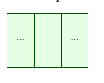
\includegraphics[width=0.2\textwidth]{stack_vert.png}\\

\subsection{Cell}

\textbf{\textbackslash cell[\textless style\textgreater]\{\textless text\textgreater\}\{\textless size\textgreater\}}: The command \textbf{\textbackslash cell} creates the structure. Multiple commands create multiple cells.\vspace{3mm}\\
\textbf{\textless style\textgreater}: The required argument \textbf{\textless style\textgreater} styles the color of the cell. The included styles include red, blue, and teal.\vspace{3mm}\\
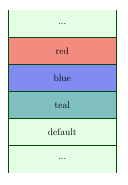
\includegraphics[width=0.2\textwidth]{stack_style.png}\\
\textbf{\textless text\textgreater}: The optional argument \textbf{\textless text\textgreater} inserts text into the cell.
\vspace{3mm}\\
\textbf{\textless size\textgreater}: The optional argument \textbf{\textless size\textgreater} sets the size of a cell in terms of number of cells. Note: this has been recently bugged, and is not working.
\subsection{Cell Addons}
Addons are commands you insert after each \textbf{\textbackslash cell}.\vspace{3mm}\\
\textbf{\textbackslash cellround\{\textless text\textgreater\}}: The command \textbf{\textbackslash cellround} addon inserts a circle annotation with text attached to an end.
\vspace{3mm}\\
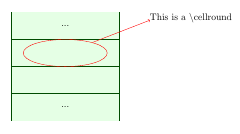
\includegraphics[width=0.4\textwidth]{stack_round.png}\\

\textbf{\textbackslash pointer\{\textless text\textgreater\}}: The command \textbf{\textbackslash pointer} addon inserts a an arrow to the right of the cell.
\vspace{3mm}\\
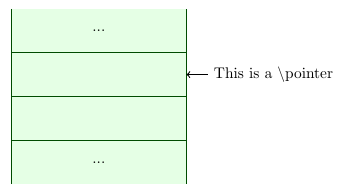
\includegraphics[width=0.4\textwidth]{stack_pointer.png}\\
\subsection{Frames}
A frame is a brace around a side of several cells. It's a decorate around the cell commands\\
\verb!\sframe!\\
\verb!  \cell!\\
\verb!  \cell!\\
\verb!\fframe{<text>}!
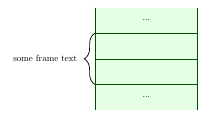
\includegraphics[width=0.4\textwidth]{stack_frame.png}

\section{LinkedLists}

\subsection{CS Singly Linked List}
Format:{\textbackslash}cslinklist[Option:styling]{\{}objects{\}}\\
Example:{\textbackslash}cslinklist{\{}a,b,c,d,e{\}} \newline \\
\begin{adjustbox}{width=0.5\paperwidth,center,keepaspectratio}
\cslinklist{a,b,c,d,e}
\end{adjustbox}\\
\subsection{CS Doubly Linked List}
Format:{\textbackslash}csdlinklist[Option:styling]{\{}objects{\}}\\
Example:{\textbackslash}csdlinklist{\{}foo,boo,coo,koo,woo,hoo{\}} \newline \\
\begin{adjustbox}{width=0.5\paperwidth,center,keepaspectratio}
\csdlinklist{foo,boo,coo,koo,woo,hoo}
\end{adjustbox}\\
\subsection{CS Circular Singly Linked List}
Format:{\textbackslash}cslooplinklist[Option:styling]{\{}objects{\}}\\
Example:{\textbackslash}cslooplinklist{\{}a,b,c,d{\}} \newline \\
\begin{adjustbox}{width=0.5\paperwidth,center,keepaspectratio}
\cslooplinklist{a,b,c,d}
\end{adjustbox}\\
\subsection{CS Circular Doubly Linked List}
Format:{\textbackslash}csloopdlinklist[Option:styling]{\{}objects{\}}\\
Example:{\textbackslash}csloopdlinklist{\{}a,b,c,d{\}} \newline \\
\begin{adjustbox}{width=0.5\paperwidth,center,keepaspectratio}
\csloopdlinklist{a,b,c,d}
\end{adjustbox}\\
%%%simple form
\subsection{Simple Singly Linked List}
Format:{\textbackslash}linklist[Option:styling]{\{}objects{\}}\\
Example:{\textbackslash}linklist{\{}a,b,c,d{\}} \newline \\
\begin{adjustbox}{width=0.5\paperwidth,center,keepaspectratio}
\linklist{a,b,c,d}
\end{adjustbox}\\

Example:{\textbackslash}linklist{\{}{\{}{\textbackslash}tikz{\textbackslash}node[draw,circle]{\{}0{\}};{\}},{\{}{\textbackslash}tikz{\textbackslash}node[draw,circle]{\{}gh{\}};{\}},{\{}{\textbackslash}tikz{\textbackslash}node[draw,circle]{\{}b{\}};{\}},{\{}{\textbackslash}tikz{\textbackslash}node[draw,circle]{\{}c{\}};{\}}{\}}\\
\begin{adjustbox}{width=0.5\paperwidth,center,keepaspectratio}
\linklist{{\tikz\node[draw,circle]{0};},{\tikz\node[draw,circle]{gh};},{\tikz\node[draw,circle]{b};},{\tikz\node[draw,circle]{c};}} 
\end{adjustbox}\\


\subsection{Simple Doubly Linked List}
Format:{\textbackslash}dlinklist[Option:styling]{\{}objects{\}}\\
Example:{\textbackslash}dlinklist{\{}a,b,c,d{\}} \newline \\
\begin{adjustbox}{width=0.5\paperwidth,center,keepaspectratio}
\dlinklist{a,b,c,d}
\end{adjustbox}\\
\subsection{Simple loop Linked List}
Format:{\textbackslash}looplinklist[Option:styling]{\{}objects{\}}\\
Example:{\textbackslash}looplinklist{\{}a,b,c,d{\}} \newline \\
\begin{adjustbox}{width=0.5\paperwidth,center,keepaspectratio}
\looplinklist{a,b,c,d}
\end{adjustbox}\\
\subsection{Simple Doubly Linked List}
Format:{\textbackslash}loopdlinklist[Option:styling]{\{}objects{\}}\\
Example:{\textbackslash}loopdlinklist{\{}a,b,c,d{\}} \newline \\
\begin{adjustbox}{width=0.5\paperwidth,center,keepaspectratio}
\loopdlinklist{a,b,c,d}
\end{adjustbox}
\newpage
\subsection{Option(Vertical): CS vs Simple: Singly and Doubly Linked Lists}

\begin{center}
\begin{adjustbox}{height=0.6\paperheight,width=\paperwidth,center,keepaspectratio}
\lrmatrix{4}{{{\textbackslash}csvdlinklist{\{}foo,boo,koo{\}}},{{\textbackslash}csvlinklist{\{}a,b,c{\}}},{{\textbackslash}vlinklist{\{}a,b,c,d,e,f,g,h,i{\}}},{{\textbackslash}dvlinklist{\{}a,b,c,d,e,f,g,h,i{\}}},\csvdlinklist{foo,boo,koo},\csvlinklist{a,b,c},\vlinklist{a,b,c,d,e,f,g,h,i},\vdlinklist{a,b,c,d,e,f,g,h,i}}
\end{adjustbox}
\end{center}
\newpage
\section{ Data Structure: HashMap Object}
Format:{\textbackslash}hashmapset[Option:styling]{\{}Name of Hashmap{\} }{\{}list of Keys{\}}{\{}list of Values{\}}\\
Example:{\textbackslash}hashmapset{\{}HashMap{\} }{\{}key1,key2,key3{\}}{\{}value1,value2,value3{\}}\newline \\
\begin{adjustbox}{width=0.5\paperwidth,center,keepaspectratio}
\hashmapset{HashMap}{key1,key2,key3}{value1,value2,value3}
\end{adjustbox}

\newpage

\section{ARRAYS:}
(Left-Right)\\ 
Format:{\textbackslash}lrmatrix{\{}number of columns to split list of objects{\} }{\{}objects{\}}\\
Example1:{\textbackslash}lrmatrix{\{}4{\} }{\{}1,2,3,4,5,6,7,a,b,c{\}}\\
Example2:{\textbackslash}lrmatrix{\{}2{\} }{\{}{\textbackslash}includegraphics{\{}ex1.jpg{\}},{\textbackslash}includegraphics{\{}ex2.jpg{\}},\\{\textbackslash}includegraphics{\{}ex3.jpg{\}},{\textbackslash}includegraphics{\{}ex4.jpg{\}}{\}}\newline

\lrmatrix{4}{1,2,3,4,5,6,7,a,b,c} \lrmatrix{2}{
\includegraphics[width=30mm]{computer_science_zoomed_by_blackblood357-d37ofou.jpg},
\includegraphics[width=30mm]{computer-science1.jpg},
\includegraphics[width=30mm]{computer-science1.jpg},
\includegraphics[width=30mm]{computer_science_zoomed_by_blackblood357-d37ofou.jpg}} \newline 

(Vertical)\\
Format:{\textbackslash}vmatrix{\{}number of rows to split list of objects{\}}{\{}objects{\}}\\
Example:{\textbackslash}vmatrix{\{}2{\}}{\{}1,2,3,4,5,6,7,a,b,c{\}}\\
\vmatrix{2}{1,2,3,4,5,6,7,a,b,c}
\newpage
\textbf{Data Structure:(Simple Hashtable)}\\
{\textbackslash}lrmatrix{\{}1{\} }{\{}\\{\textbackslash}linklist{\{}{\{}{\textbackslash}tikz{\textbackslash}node[draw,circle]{\{}0{\}};{\}},a,b,c{\}},\\{\textbackslash}linklist{\{}{\{}{\textbackslash}tikz{\textbackslash}node[draw,circle]{\{}1{\}};{\}},d,e,f{\}},\\{\textbackslash}linklist{\{}{\{}{\textbackslash}tikz{\textbackslash}node[draw,circle]{\{}0{\}};{\}},g,h,i{\}}{\}}\newline \\
\lrmatrix{1}{\linklist{{\tikz\node[draw,circle]{0};},a,b,c},\linklist{{\tikz\node[draw,circle]{1};},d,e,f},\linklist{{\tikz\node[draw,circle]{2};},g,h,i}}

\section{Object Diagramming}
Format:\\
{\textbackslash}begin{\{}diagram{\}}{\{}Styling{\}}\\ 
-----Content------\\
{\textbackslash}end{\{}diagram{\}}\\
\subsection{Example: Class Diagram}
Format:\\
{\textbackslash}class[Option: styling]{\{}class var{\}}[Option:Title][Option:members][Option:operations]\\
{\textbackslash}rel{\{}relationship{\}}{\{}derive source{\}} {\{}deriver{\}}\\
EX:
{\textbackslash}begin{\{}diagram{\}}{\{}node distance=5cm,layered layout{\}}\\
{\textbackslash}class[rounded corners, fill=red!20]{\{}a{\}}[Interface{\textbackslash}{\textbackslash}Classes][members][operations]\\
{\textbackslash}class[rounded corners, fill=blue!20]{\{}b{\}}[class1][members][operations]\\
{\textbackslash}class{\{}c{\}}[class2][members][operations]\\
{\textbackslash}class{\{}d{\}}[class3][members]\\
{\textbackslash}class[rounded corners]{\{}e{\}}[other Object][members][operations]\\
{\textbackslash}rel{\{}generalization{\}}{\{}a{\}} {\{}b,c,d{\}}\\
{\textbackslash}rel{\{}dependency{\}}{\{}e{\}}{\{}d{\}}\\  
{\textbackslash}end{\{}diagram{\}}\\

\begin{diagram}{node distance=5cm,layered layout}
\class[rounded corners, fill=red!20]{a}[Interface\\Classes][members][operations]
\class[rounded corners, fill=blue!20]{b}[class1][members][operations]
\class{c}[class2][members][operations]
\class{d}[class3][members]
\class[rounded corners]{e}[other Object][members][operations]
\rel{generalization}{a} {b,c,d}
\rel{dependency}{e}{d}
    
\end{diagram}

\section{Limitations}
\subsection{object diagrams}

Object diagramming is dependent on LuaTex. Its layouts are derived from the gdlibrary of the tikz package(implemented with LuaTex).\\ \newline

If using a custom Tikz object within the diagram environment, a nested tikz node will not be seen and will be treated as an empty object.\\ \newline

Reference objects are always anchored parallel to its associated node. If size of object is larger than the default distance of hashmap nodes, reference object(s) will overlap each other.(No automatic spacing). Fix by manually changing the node distance in option:styling parameter(ex:node distance=x), and/or scale the reference object. \\ \newline

\vspace{3mm}

\section{Bugs and Solutions}
\subsection{File Names Not Recognized}
\LaTeX has problems with dot filenames.
Example:  sp2.0b.dvi. Latex sees the .0b.dvi as the entire extension. It should only see .dvi as the extension.\\
Solution
Add \verb!\usepackage{grffile}! to handle dot filenames.
\subsection{Empty Figures, indexes, ToC, etc.}
You need to compile twice (sometimes three times). For an automated solution, see:  http://www.ctan.org/pkg/latexmk.
\clearpage
\subsection{Suggested Template with Packages}
\verb!\documentclass[openany]{book}!\\
\verb!\RequirePackage{cmds}!\\
\verb!\RequirePackage{graphicx}!\\
\verb!\RequirePackage{epstopdf}!\\
\verb!\RequirePackage{grffile}!\\
\verb!\usepackage[T1]{fontenc}!\\
\verb!\RequirePackage{makeidx}!\\
\verb!\RequirePackage[linktoc=all]{hyperref}!\\
\verb!\hypersetup{!\\
\verb!    colorlinks,!\\
\verb!    citecolor=black,!\\
\verb!    filecolor=black,!\\
\verb!    linkcolor=black,!\\
\verb!    urlcolor=black!\\
\verb!}!\\
\verb!!\\
\verb!\begin{document}!\\
\verb!\tableofcontents!\\
\verb!\listoffigures	% optional!\\
\verb!\listoftables	% optional!\\
\verb!\end{document}!\\
\subsection{Explanation of Packages}
\textbf{graphicx}\vspace{3mm}
Allows insertion of JPG, PNG, PDF, EPS into document.\\
\textbf{epstopdf}\vspace{3mm}
Required for EPS support (with use of pdflatex command).\\
\textbf{grffile}\vspace{3mm}
Required for complex filenames (see bug section).\\
\textbf{hyperref}\vspace{3mm}
Enables the toc to hyperlink to the correct parts.  It can be [=none, section, page, all].\\
\end{document}

